\documentclass[]{standalone}

\usepackage{amsmath}
\usepackage{amsfonts}
\usepackage{amssymb}
\usepackage{graphicx}
\usepackage{tikz}
\usepackage{import}
\usepackage[subpreambles=true]{standalone}

\usepackage{tikz}
\usepackage{tikz-3dplot}

\usetikzlibrary{positioning}
\usetikzlibrary{calc}
\begin{document}

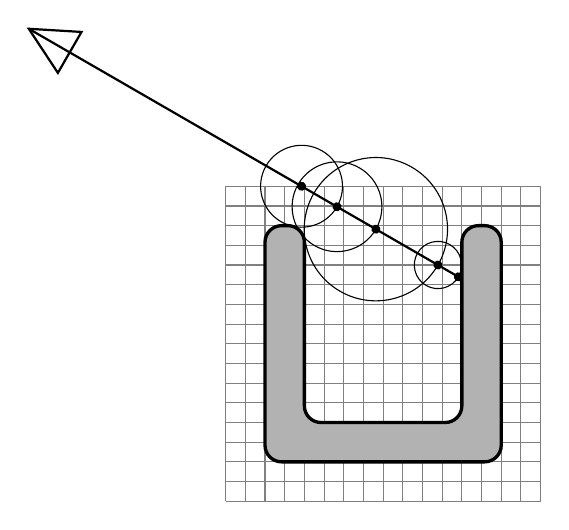
\begin{tikzpicture}[scale=1]

\coordinate (camera) at (0, 2.5);
\coordinate (object) at (3.0, 0);
\coordinate (grid) at (2.5, 0.5);

\draw[step=0.25cm,black,thin,xshift=0.0cm,yshift=0.0cm,gray] ($(grid)-(0.001,-0.001)$) grid ++(4.001,-4.001);
% \def\d1{0.5}

\begin{scope} [rotate=-30,shift={(camera)}]
    \path[draw, thick] (0,0) -- (6.5,0);
    \path[draw, thick] (0,0) -- (0.6,0.3) -- (0.6, -0.3) -- cycle;

    \path[draw, fill] (4.0,0) circle (0.05);
    \path[draw] (4.0,0) circle (0.52);
    \path[draw, fill] (4.52,0) circle (0.05);
    \path[draw] (4.52,0) circle (0.57);
    \path[draw, fill] (5.09,0) circle (0.05);
    \path[draw] (5.09,0) circle (0.91);
    \path[draw, fill] (6.0,0) circle (0.05);
    \path[draw] (6.0,0) circle (0.3);
    \path[draw, fill] (6.3,0) circle (0.05);
    % \node [transform shape](scope6) at (0,0) {\includegraphics{example-image}}; 
    % \node at (0,0) [rotate=0,color=black] {Text};
\end{scope}

    \path[draw, very thick, rounded corners=6pt, fill=black!30] (object) -- ++(0.5,00) -- ++(0,-2.5) -- ++(2.0, 0) -- ++(0,2.5) -- ++(0.5,0) -- ++(0,-3.0) -- ++(-3.0,0) -- cycle;


\end{tikzpicture}
\end{document}
